\documentclass[12pt,a4paper]{article}
\usepackage{rmpackages}																% usual packages
\usepackage{rmtemplate}																% graphic charter
\usepackage{rmexocptce}																% for DS with cptce eval

\newcounter{memory}

\begin{document}

\begin{header}
Devoir surveillé
\normalsize
\flushleft
\begin{doublespace}
Classe :

NOM :

\end{doublespace}
Prénom :
\end{header}
L'énoncé est à rendre avec la copie : indiquez vos nom et prénom sur l'énoncé.

\noindent
La rédaction et la propreté de la copie (tenue, mise en valeur des résultats, orthographe) seront valorisées dans la notation.

\noindent
\com{} \ajcom{0.75}

\begin{exo}{Cours}

\begin{enumerate}
\item \rco{} \ajrco{1.5}

Parmi les deux formules ci-dessous, laquelle permet de calculer la concentration massique $C_\mathrm{m}$ d'une solution.
Rappeler l'unité de \textbf{toutes} les grandeurs.
À quelle grandeur correspond l'autre formule ?
\begin{multicols}{3}
\begin{enumerate}
\item $\frac{m_\mathrm{soluté}}{V_\mathrm{solution}}$

\item $\frac{m_\mathrm{solution}}{V_\mathrm{solution}}$
\end{enumerate}
\end{multicols}

\begin{multicols}{2}
\item \anarai{} \ajanarai{1}

Donner le nom de la manipulation réalisée avec le matériel ci-contre.

\item \rco{} \ajrco{0.5}

Donner le nom du récipient le plus à droite sur le schéma.
\begin{center}
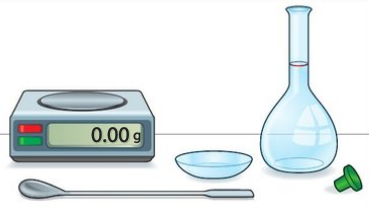
\includegraphics[scale=1]{images/materiel_dissolution.png}
\end{center}
\end{multicols}

\item \rco{} \ajrco {0.5} \rea{} \ajrea{0.5}

Donner la taille d'un atome en nanomètre, puis en mètre en utilisant les puissances de 10.

\item \rco{} \ajrco{1.25}

Associer chaque formule chimique au bon terme parmi : atome, molécule, cation, anion.
\begin{multicols}{5}
\begin{itemize}
\item[•] $\permanganate$
\item[•] $\text{O}$
\item[•] $\ionmagnesiumII$
\item[•] $\acideoleique$
\item[•] $\dioxydedecarbone$
\end{itemize}
\end{multicols}


\end{enumerate}

\end{exo}

\newpage

\begin{exo}{Solution sucrée pour sportif}

Les boissons isotoniques pour sportifs contiennent environ \unit{6}{g} de sucre pour \unit{100}{mL} de solution.

Un sportif remplit sa gourde, de volume \unit{0{,}75}{L}, avec une solution isotonique notée $\mathrm{S_1}$. Après plusieurs heures de sport, le sportif a bu les deux tiers du contenu de sa gourde. Il la complète avec de l'eau et obtient une nouvelle solution notée $\mathrm{S_2}$.

\begin{enumerate}
\item \app{} \ajapp{0.5}

Dans la solution isotonique, identifier le soluté. 

\item \app{} \ajapp{0.5} \rea{} \ajrea{1.5}

Calculer la concentration en masse en sucre de la solution isotonique $\mathrm{S_1}$.
La formule littérale et le détail des conversions sont attendus.

\item \rea{} \ajrea{0.5}

Calculer le volume de solution restant dans la gourde quand le sportif en a bu les deux tiers.

\item \rea{} \ajrea{1.5}

Déterminer la masse de sucre dans la gourde quand le sportif a bu les deux tiers de son contenu.
La formule littérale et le détail des conversions sont attendus.

\item \app{} \ajapp{0.5}

Donner le volume de la solution $\mathrm{S_2}$.

\item \rea{} \ajrea{1.5}
\label{quest:C2}

En déduire la concentration en masse en sucre de la solution $\mathrm{S_2}$.
La formule littérale et le détail des conversions sont attendus.

\item \app{} \ajapp{0.5}

Donner le nom de la manipulation réalisée pour préparer la solution $\mathrm{S_2}$.

\end{enumerate}

La boisson isotonique contient aussi des colorants alimentaires pour rendre la boisson plus attrayante.
À partir de la solution isotonique $\mathrm{S_1}$, on réalise l'échelle de teinte visible ci-dessous.
La concentration en sucre de chaque solution est connue et indiquée au dessus de chaque solution.
Pour l'analyser, un échantillon de la solution $\mathrm{S_2}$ est prélevé dans la gourde du sportif.

\begin{enumerate}[resume]
\item \anarai{} \ajanarai{1} \val{} \ajval{0.5}

Le résultat trouvé à la question~\ref{quest:C2} est-il en accord avec cette analyse ?
Justifier.
\end{enumerate}

\begin{center}
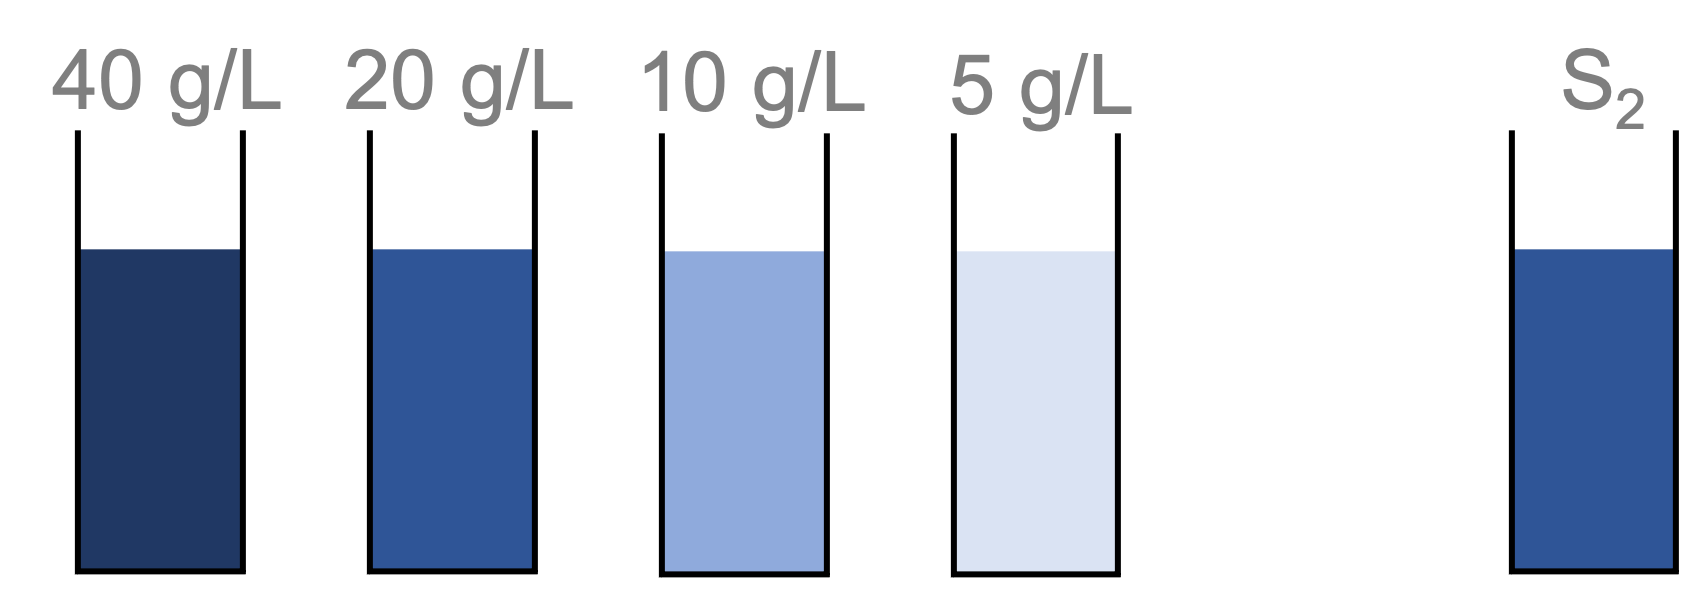
\includegraphics[scale=0.5]{images/echelle_teinte_isotonique.png}
\end{center}

\end{exo}

\newpage

\begin{exo}{La planète rouge}

\begin{multicols}{2}
\begin{center}
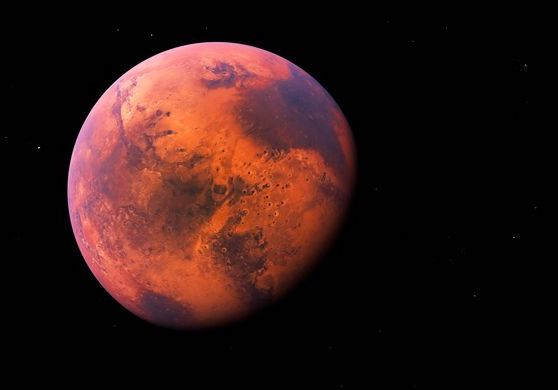
\includegraphics[scale=0.4]{images/mars.jpg}
\end{center}

La couleur rouge de la surface de Mars est due, entre autres, à la présence d'oxyde de fer de formule $\oxydedefer$.
Ce composé est formé des ions fer $\ionferIII$ et des ions $\oxyde$.

\begin{enumerate}
\item \app{} \ajapp{1}

Parmi les ions qui composent l'oxyde de fer, identifier le cation et l'anion.

\item \anarai{} \ajanarai{1}

\com{} \ajcom{0.5}

Justifier la formule de l'oxyde de fer.
\setcounter{memory}{\theenumi}
\end{enumerate}
\end{multicols}

Certains composés témoignent de la présence passée d'eau sur Mars.
C'est le cas des chlorures et des sulfates identifiés à l'emplacement d'anciens lacs et rivières, maintenant disparus.

\begin{multicols}{2}
\begin{enumerate}
\setcounter{enumi}{\thememory}
\item \anarai{} \ajanarai{1}

Donner la formule du chlorure de sodium.

\item \anarai{} \ajanarai{1}

Donner la formule du sulfate de calcium.

\item \anarai{} \ajanarai{1}

Donner la formule de l'ion magnésium présent dans le sulfate de magnésium de formule $\text{MgSO}_\text{4}$.
\end{enumerate}

\hfill
\begin{center}
\begin{tabular}{l | c}
\textbf{Nom} & \textbf{Formule chimique} \\
\hline\hline
ion chlorure		& $\chlorure$ \\
ion sulfate			& $\sulfate$ \\
ion carbonate	& $\carbonate$ \\
ion potassium 	& $\ionpotassium$ \\
ion sodium     	& $\ionsodium$ \\
ion calcium		& $\ioncalcium$ \\
\end{tabular}
\end{center}

\end{multicols}

\end{exo}

\vfill
\makecptces

\end{document}